\section{Introdução e Estudo de Caso (Swain vs. Alabama)}

\begin{frame}{O Problema da Decisão com Dados}
    \begin{block}{Pergunta Fundamental}
        Como avaliar se uma discrepância observada em nossos dados é real (sinal sistemático) ou se é apenas fruto da variabilidade natural do acaso (ruído aleatório)?
    \end{block}
    \begin{block}{Exemplos Anteriores}
        \begin{itemize}
            \item Eficácia de vacinas em ensaios clínicos.
            \item Probabilidade em lançamentos de moedas.
            \item Diferença de peso de recém-nascidos.
        \end{itemize}
    \end{block}
    \centering
    \textit{Hoje exploraremos uma abordagem computacional robusta baseada em simulação e reamostragem para responder a essa pergunta de forma intuitiva.}
\end{frame}

\begin{frame}{Estudo de Caso: Robert Swain vs. Alabama (1962)}
    \begin{block}{O Contexto Histórico}
        Em 1962, Robert Swain, um homem negro, foi condenado à morte no Alabama. Ele apelou da sentença apontando que o júri era inteiramente branco e denunciou discriminação racial sistemática no processo de seleção.
    \end{block}
    \begin{columns}
        \begin{column}{0.6\textwidth}
            \textbf{Dados Demográficos do Caso:}
            \begin{itemize}
                \item População de jurados elegíveis: $26\%$ negros.
                \item Painel de pré-seleção ($N$): $100$ homens.
                \item Quantidade de negros no painel ($X$): apenas $8$ ($8\%$).
                \item Júri final da condenação: $0$ negros.
            \end{itemize}
        \end{column}
        \begin{column}{0.4\textwidth}
            \centering
            \textit{A Suprema Corte americana negou o apelo afirmando que a discrepância era pequena.}
        \end{column}
    \end{columns}
\end{frame}

\begin{frame}{Relembrando: Intervalo de Confiança Clássico (TCL)}
    \begin{columns}
        \begin{column}{0.5\textwidth}
            \begin{block}{Parâmetros da Amostra}
                \begin{itemize}
                    \item $N = 100$ jurados.
                    \item $p = 0.08$ ($8\%$ negros).
                \end{itemize}
            \end{block}
            \begin{block}{Variância de Bernoulli}
                $X_i \in \{0, 1\}$ (V.A. de Bernoulli):
                \begin{itemize}
                    \item Média ($\bar{X}$) = $p = 0.08$
                    \item Variância ($s^2$) = $p(1 - p) = 0.0736$
                    \item Erro Padrão ($SE$) = $\sqrt{\frac{p(1 - p)}{N}} \approx 0.0271$
                \end{itemize}
            \end{block}
        \end{column}
        \begin{column}{0.5\textwidth}
            \begin{alertblock}{Cálculo do $IC_{95\%}$ via TCL}
                $$IC_{95\%} = p \pm z \times SE$$
                $$IC_{95\%} = 0.08 \pm 1.96 \times 0.0271$$
                $$IC_{95\%} = 0.08 \pm 0.0531$$
                $$IC_{95\%} = [2.69\%; 13.31\%]$$
                \vspace{0.1cm}
                {\footnotesize \textit{A proporção esperada de $26\%$ está completamente fora do intervalo!}}
            \end{alertblock}
        \end{column}
    \end{columns}
\end{frame}

\begin{frame}[fragile]{Relembrando: Intervalo de Confiança via Bootstrap}
    \begin{block}{Abordagem de Reamostragem (Bootstrap)}
        Se não quisermos assumir a aproximação normal do TCL, podemos reamostrar com reposição a partir da própria amostra original de $100$ pessoas ($8$ negros e $92$ brancos).
    \end{block}
\begin{lstlisting}[language=Python]
import numpy as np

# Amostra original: 1 para negro, 0 para branco
amostra = np.array([1]*8 + [0]*92)

# Gera 10.000 amostras Bootstrap de tamanho 100 com reposicao
np.random.seed(42)
medias_boot = [np.random.choice(amostra, size=100).mean() for _ in range(10000)]

# Intervalo de Confianca de 95% (Percentis 2.5% e 97.5%)
ic_inf = np.percentile(medias_boot, 2.5)
ic_sup = np.percentile(medias_boot, 97.5)
print(f"IC 95% Bootstrap: [{ic_inf:.4f}; {ic_sup:.4f}]")
# Saida: [0.0300; 0.1400] (ou [3.0%; 14.0%])
\end{lstlisting}
    \centering
    \vspace{0.1cm}
    \textit{Novamente, a proporção esperada de $26\%$ está fora do intervalo!}
\end{frame}


\begin{frame}{Modelando o Acaso (Modelo Nulo)}
    \begin{block}{Definição de Modelo Nulo}
        É uma suposição básica de que não há efeito sistemático; qualquer diferença observada é puro fruto do acaso. Conseguimos programar computacionalmente esse modelo.
    \end{block}
    \begin{block}{Nosso Exemplo:}
        Cada pessoa do painel é selecionada de forma independente, com probabilidade constante $\mu = 0.26$ de ser negra. O júri é uma amostra de tamanho $N = 100$.
    \end{block}
    \begin{alertblock}{A Pergunta Estatística}
        Qual a probabilidade de selecionar $8$ ou menos homens negros em um painel aleatório de $100$ pessoas, quando a proporção real na população é de $26\%$?
    \end{alertblock}
\end{frame}

\begin{frame}[fragile]{Construindo o Modelo Simulado: População}
    \begin{block}{Ideia de Simulação Física}
        Para comparar nossos dados com o modelo aleatório, podemos simular toda a população do município em um vetor.
        \begin{itemize}
            \item Definimos uma população grande (ex: $10.000$ pessoas).
            \item Seta todos para `'W'` (Branco).
            \item Seta os primeiros $26\%$ para `'B'` (Negro), representando a hipótese nula $H_0$.
        \end{itemize}
    \end{block}
\begin{lstlisting}[language=Python]
import numpy as np
pop_total = 10000
prop_negros = 0.26

# Cria o vetor da populacao e seta todos para 'W'
populacao = np.zeros(shape=pop_total, dtype='c')
populacao[:] = 'W'

# Seta os primeiros 26% para 'B'
populacao[:int(pop_total * prop_negros)] = 'B'
\end{lstlisting}
    \centering
    \vspace{0.1cm}
    \textit{Note que essa simulação é conceitualmente a mesma coisa do Bootstrap, mas aqui simulamos a população!}
\end{frame}

\begin{frame}[fragile]{Como Simular o Sorteio do Júri?}
    \begin{block}{Algoritmo de Simulação por Embaralhamento}
        Para simular a seleção justa de um júri de $100$ pessoas:
        \begin{enumerate}
            \item Embaralhe a população aleatoriamente.
            \item Selecione os primeiros $100$ elementos como o júri.
            \item Conte e guarde o número de negros.
            \item Repita o processo $10.000$ vezes.
        \end{enumerate}
    \end{block}
\begin{lstlisting}[language=Python]
juri_tamanho = 100
repeticoes = 10000
simulacoes = np.zeros(repeticoes)

for i in range(repeticoes):
    np.random.shuffle(populacao)
    juri = populacao[:juri_tamanho]
    num_negros = (juri == b'B').sum()
    simulacoes[i] = num_negros
\end{lstlisting}
    \centering
    \vspace{0.1cm}
    \textit{Embora muito visual, este método é lento. Usamos a distribuição Binomial para simular o mesmo processo de forma otimizada!}
\end{frame}


\begin{frame}[fragile]{Abordagem Computacional: Simulação Monte Carlo}
\begin{lstlisting}[language=Python]
import numpy as np

# Proporcao populacional de negros (Hipotese Nula)
prob_negros = 0.26
tamanho_painel = 100
repeticoes = 10000

# Simula 10000 paineis usando a distribuicao Binomial
np.random.seed(42)
simulacoes = np.random.binomial(n=tamanho_painel, p=prob_negros, size=repeticoes)

# Calcula a proporcao de paineis com 8 ou menos negros
p_valor = np.count_nonzero(simulacoes <= 8) / repeticoes
print(f"P-valor simulado: {p_valor:.6f}")
# Saida esperada: 0.000000
\end{lstlisting}
\end{frame}

\begin{frame}{Tomada de Decisão Visual}
    \begin{columns}
        \begin{column}{0.5\textwidth}
            \textbf{Análise do Histograma:}
            \begin{itemize}
                \item Os valores simulados sob a hipótese nula variam em torno de $26$.
                \item Em $10.000$ simulações, o menor valor gerado foi acima de $12$.
                \item O valor observado de $8$ negros é extremamente raro (probabilidade praticamente zero).
                \item \textbf{Decisão:} Rejeitamos o modelo de seleção justa.
            \end{itemize}
        \end{column}
        \begin{column}{0.5\textwidth}
            \centering
            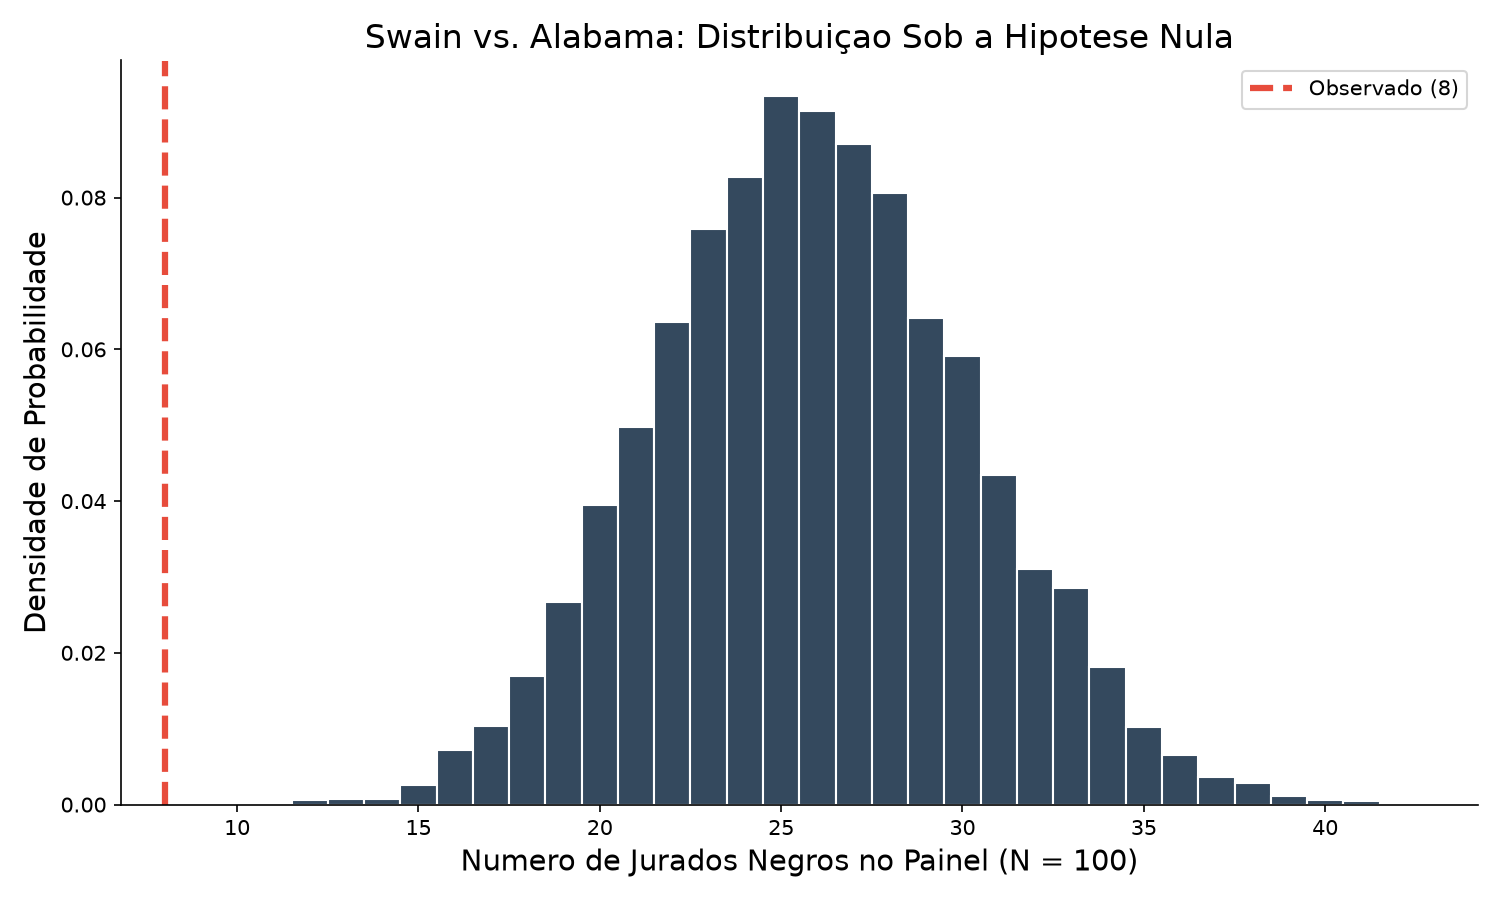
\includegraphics[width=\textwidth]{01_swain_histograma.png}
        \end{column}
    \end{columns}
\end{frame}
